\section{The Rust Model}
\thispagestyle{plain} % surpress header on first page

This section follows up on the previous one in the sense that it introduces the model created by \cite{Rust.1987} and presents how NFXP and MPEC can be used to estimate its model parameters. My notation is mainly inspired by the one employed in \cite{Su.Judd.2012}.

\subsection{The Economic Model}

Rust's model is based on the decision making process of Harold Zurcher who is in charge of a bus fleet and has to decide in each month $t = 0, 1, 2, ...$ whether to replace the engine ($d^i_t=1$) of one or more buses $i = 1, 2, ..., M$ in his fleet or otherwise repair them in a less costly way ($d^i_t=0$). The agent, hence, chooses from the discrete action space $\mathcal{D} = \{0, 1\}$. This choice is assumed to be independent across buses and Zurcher bases his decision on two state variables which are the observed cumulative mileage $x^i_t$ of a bus since the last engine replacement and some unobserved (by the econometrician) factor $\epsilon^i_t$. The state of a bus $i$ in period $t$ is therefore fully described by ($x^i_t$, $\epsilon^i_t$) $\in \mathcal{S}$ with $\mathcal{S}$ being the state space. The agent receives an immediate reward in period $t$ from the chosen replacement decision $d^i_t(x^i_t, \epsilon^i_t)$. The choice in turn affects the possible state space $\mathcal{S'}$ in the period $t+1$ as the cumulative mileage after replacement $x^i_{t+1}$ depends on the choice of $d^i_t$. The decision problem is essentially regenerative as the mileage state is set back to zero after the decision to replace the engine of a bus. As the agent is forward looking with a discount factor $\beta \in (0, 1)$ he does not simply maximize the immediate reward but rather the expected discounted utility over an infinite horizon with a higher preference for reward occurring closer to the present. The immediate reward is additively separable can be characterized in the following way:

\begin{equation}
	u(x^i_t, d^i_t, \epsilon^i_t; \theta_1, RC) = v(x^i_t, d^i_t; \theta_1, RC) + \epsilon^i_t
\end{equation}

with

\[v(x^i_t, d^i_t; \theta_1, RC) = \left\{
\begin{array}{lr}
-c(x; \theta_1)  & \mbox{if } d^i_t = 0 \\
-RC -c(0;\theta_1) & \mbox{if } d^i_t = 1
\end{array}
\right.
\]

The immediate reward is hence determined by some operating cost $c(.)$ that is assumed to be increasing in the cumulative mileage state $x$ if regular maintenance as opposed to engine replacement is chosen. If replacement is picked it consists of a replacement cost $RC$ and the operating cost $c(.)$ after resetting the cumulative mileage to zero. This shows that the choice of the agent $d^i_t$ depends crucially on the structural cost parameters $\theta_1$ and $RC$ that define the exact shape of the cost function. The timing of events for a single bus in the decision process of Harold Zurcher is depicted in Figure \ref{Figure1} below.
\paragraph{}

\begin{figure}[H]
	\caption{\label{Figure1}Timing of the Decision Model}
	\vspace{2ex}
	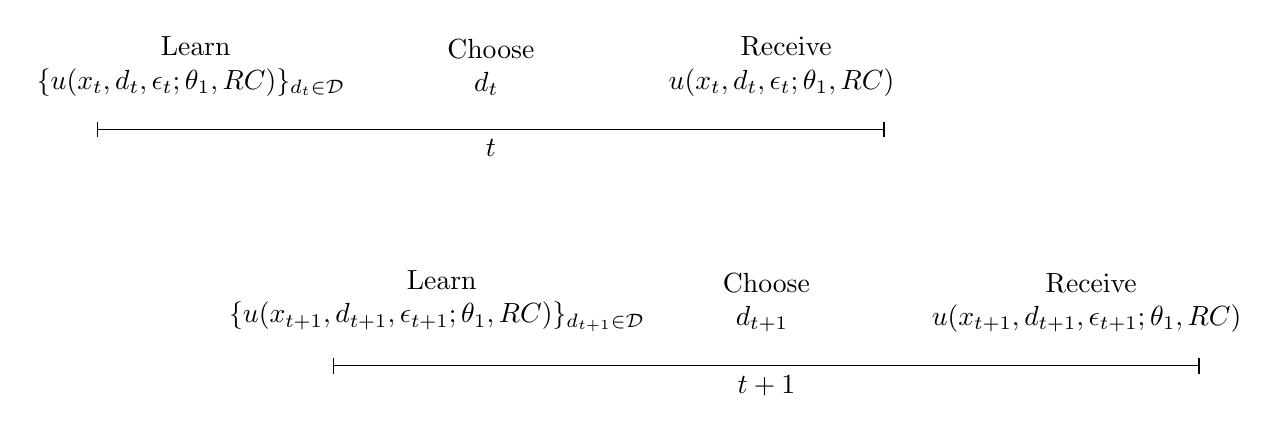
\begin{tikzpicture}
	\draw [|-|]
	(0,1) -- (10,1)
	node [above,align=center,very near start]
	{
		Learn\\
		$\{u(x_t, d_t, \epsilon_t; \theta_1, RC)\}_{d_t \in \mathcal{D}}$
		\vspace{2ex}
	}
	node [above,align=center,midway]
	{
		Choose\\
		$d_t$
		\vspace{2ex}
	}
	node [above,align=center,very near end]
	{
		Receive\\
		$u(x_t, d_t, \epsilon_t; \theta_1, RC)$
		\vspace{2ex}
	}
	node [below, align=center, midway]
	{$t$};
	\draw [|-|]
	(3,-2) -- (14,-2)
	node [above,align=center,very near start]
	{
		Learn\\
		$\{u(x_{t+1}, d_{t+1}, \epsilon_{t+1}; \theta_1, RC)\}_{d_{t+1} \in \mathcal{D}}$
		\vspace{2ex}
	}
	node [above,align=center,midway]
	{
		Choose\\
		$d_{t+1}$
		\vspace{2ex}
	}
	node [above,align=center,very near end]
	{
		Receive\\
		$u(x_{t+1}, d_{t+1}, \epsilon_{t+1}; \theta_1, RC)$
		\vspace{2ex}
	}
	node [below, align=center, midway]
	{$t+1$};

	\end{tikzpicture}
\end{figure}
\vspace{2.5ex}

The transition of the state vector ($x^i_t$, $\epsilon^i_t$) is assumed to follow a Markov process, i.e. the current state only depends on the previous one and hence the utility maximization problem is time-invariant. This means that the problem faced by Zurcher is the same for a given state $(x^i_t$, $\epsilon^i_t)$ irrespective of the time $t$ in which he has to make his choice. Dropping the bus index $i$ for convenience, the optimization problem of the agent gives rise to the following value function for a single bus:

\begin{equation}
V(x_t, \epsilon_t) = \max_{\{d_t, d_{t+1}, ... \}} \E \left[\sum_{\tau=t}^{\infty} \beta^{\tau - t} u(x_\tau, d_\tau, \epsilon_\tau; \theta_1, RC)\right]
\end{equation}

Solving this model leads to an optimal policy rule $\pi^* = (d^{\pi^*}_t(x_t, \epsilon_t))^\infty_t$.

\subsection{The Model Solving}

The solution to the above model can be characterized by the Bellman equation (\cite{Bellman.1954}) below:

\begin{equation}
	\begin{split}
		V(x, \epsilon) = &\max_{d} \{v(x, d; \theta_1, RC) + \epsilon(d) \\[+3mm]
		&+ \beta \int_{x'} \int_{\epsilon'} V(x', \epsilon') p(x', \epsilon'| x, \epsilon, d, \theta_2, \theta_3) dx' d\epsilon'\}
	\end{split}
\end{equation}

with $(x, \epsilon)$ being the current period and $(x', \epsilon')$ the next period state. \paragraph{}

\cite{Rust.1987} simplifies the above problem now by assuming \textit{conditional independence} on the transition probabilities of the state vector $p(.)$:

\begin{equation}
	p(x', \epsilon'| x, \epsilon, d, \theta_2, \theta_3) = p_2(\epsilon'|x';\theta_2)p_3(x'|x, d; \theta_3)
\end{equation}

with further assuming that $\epsilon(d)$ is following a bivariate i.i.d. extreme value distribution with $\theta_2$ being Euler's constant. \paragraph{}

After discretizing the possible, continuous values of the state variable $x$, Rust derives from the original Bellman equation above the following contraction mapping needed to solve the economic model:

\begin{equation}
	\label{eq9}
	\begin{split}
		EV(\hat x_k, d) = &\sum_{j=0}^{J} log \left\{ \sum_{d'\in\{0, 1\}}  exp[v(x', d'; \theta_1, RC) + \beta EV(x', d')]\right\} \\[+3mm]
		&\times p_3(x'|\hat x_k, d; \theta_3).
	\end{split}
\end{equation}

with

\[p_3(x'|\hat x_k, d; \theta_3) = \left\{
\begin{array}{lr}
	Pr\{x'=\hat x_{k+j}|\theta_3\}  & \mbox{if } d = 0 \\
	Pr\{x'=\hat x_{1+j}|\theta_3\} & \mbox{if } d = 1
\end{array}
\right.
\]

for $j=0, 1, ..., J$ indicating how many grid points the mileage state climbs up in the next period. \paragraph{}

In the above equation, $EV(.)$ denotes the unique fixed point to a contraction mapping $T_f(EV, \theta)$ on the full state space $\Gamma_f = \{(\hat x_k, d)|\hat x_k \in \mathbf{\hat x}, d \in \mathcal{D}\}$. Here, $\hat x_k$ represents the grid point $k$ of the state variable $x$ while $\hat x_1 = 0$. The number of possible $\hat x_k$ depends on the choice of the grid size $K$ set by the researcher. The set of possible grid points then is denoted as $\mathbf{\hat x} = \{\hat x_1, ..., \hat x_K\}$. All the variables $v$ depict current period variables while variables $v'$ display the possible value in the next period. The conditional probability function $p_3(.)$ indicates how likely it is that a bus moves up a specific amount of grid points in the next period depending on the structural parameter $\theta_3$ as well as the choice $d$. Imagine now we decide to set the grid size to $K=90$ as done in \cite{Rust.1987}, then we generally have to find the fixed point above which yields the solution $EV_f = (EV(\hat x_1, 0), ..., EV(\hat x_{90}, 0), EV(\hat x_1, 1), ..., EV(\hat x_{90}, 1))$. This simplifies, though, as all the expected values from $EV(\hat x_1, 1), ..., EV(\hat x_{90}, 1)$ are actually equivalent to $EV(\hat x_1, 0)$ due to the regenerative nature of the decision problem. This means that in our scenario we just have to solve the vector $(EV(\hat x_1, 0)\; ...\; EV(\hat x_K, 0))^T$ which I denote as $EV_r$ and we have the whole vector $EV_f$ at hand. In our example the vector $EV_r$ has a dimension of $90$. This observation will later be important for the difference between NFXP and MPEC. \cite{Su.Judd.2012}, hence, denote the dimension-reduced contraction mapping shorthand as:

\begin{equation}
EV_r = T_r(EV_r, \theta)
\end{equation}

with $T_r(.)$ being a contraction mapping on the reduced state space $\Gamma_r = \{(\hat x_k, d=0)|\hat x_k \in \mathbf{\hat x}\}$.

The unique fixed point can now be used to derive conditional choice probabilities of the agent:

\begin{equation}
	\label{eq11}
	P(d|\hat x; \theta) = \frac{exp[v(\hat x, d; \theta_1, RC) + \beta EV(\hat x, d)]}{\sum_{d' \in \{0, 1\}} exp[v(\hat x, d'; \theta_1, RC) + \beta EV(\hat x, d')]}.
\end{equation}

The above equation describes the probability that the agent chooses $d$ given that the observed mileage state is at a certain grid point $\hat x$. This derivation depends on both the cost parameters ($\theta_1$, $RC$) directly and indirectly through $EV(.)$ as well as on the transition parameter $\theta_3$. These conditional choice probabilities together with the transition probabilities $p_3(.)$ become relevant in the next section when calibrating the model using maximum likelihood.


\subsection{Calibration}

In order to calibrate the parameter vector $\theta =(\theta_1, \theta_3, RC)$ using either NFXP or MPEC, let us assume that we observe some data set $X = (X^i)^M_{i=1 }$ with $X^i = (x^i_t, d^i_t)^T_{t=1}$ for a single bus $i = 1, ..., M$. The data therefore consists of the engine replacement decision per bus and period as well as the cumulative mileage since the last engine replacement. The cumulative mileage $x^i_t$ is assumed to already be discretized which means that it takes values on the grid $\mathbf{\hat x} = \{\hat x_1, ..., \hat x_K\}$. The log likelihood of observing the data $X$ now becomes:

\begin{equation}
	L(\theta) = \sum_{i=1}^{M} \sum_{t=2}^{T} log[P(d^i_t|x^i_t; \theta)] + \sum_{i=1}^{M} \sum_{t=2}^{T} log[p_3(x^i_t|x^i_{t-1}, d^i_{t-1}; \theta_3)].
\end{equation}

To fulfill the aim of finding the optimal parameter vector $\theta$ one now has to solve the problem of maximizing the above log likelihood:

\begin{equation}
	\max_{\theta} L(\theta).
\end{equation}

The path taken by the NFXP is now to hand this unconstrained optimization problem to an optimization algorithm such as the Berndt-Hall-Hall-Hausman (BHHH) algorithm based on \cite{Berndt.1974}. The algorithm comes up with a guess for the optimal parameter $\hat \theta$ for which in a subroutine the expected values in equation \ref{eq9} are calculated. The expected value function is in turn needed to obtain the conditional choice probabilities in equation \ref{eq11} which are then taken to evaluate the log likelihood $L(\theta)$. Based on this evaluation, the optimization algorithm comes up with a new guess for $\hat \theta$ and the above procedure is repeated until a certain convergence criteria of the algorithm is met. This procedure is again shown in pseudocode in Algorithm \ref{alg3} on the next page.

At every structural guess of the optimization algorithm the fixed point $EV(.)$ is calculated precisely as it is needed to evaluate the log likelihood $L(\theta)$. This is deemed inefficient by \citeauthor{Su.Judd.2012} which gives rise to the augmented log likelihood mentioned before for which they insert the conditional choice probabilities $P(d^i_t|x^i_t; \theta)$ into $L(\theta)$ making the log likelihood explicitly depend on $EV(.)$. This results in the following log likelihood:

\vspace{2ex}
\begin{algorithm}[!h]
	\caption{Nested Fixed Point Algorithm for the Rust Model}
	\label{alg3}
	\SetAlgoLined
	\KwIn{$\hat\theta_n$, $n=0$, $X$\;}
	\While{$f(|| (\hat\theta_{n+1}, \hat{EV}_{n+1}) - (\hat\theta_{n}, \hat{EV}_{n}) ||) \geq$ stopping tolerance}{
		\vspace{2ex}
		Solve fixed point
		\begin{equation*}
		EV(\hat x_k, d) = \sum_{j=0}^{J} log \left\{ \sum_{d'\in\{0, 1\}}  exp[v(x', d'; \hat \theta_{n, 1}, \hat{RC_n}) + \beta EV(x', d')]\right\} \times p_3(x'|\hat x_k, d; \hat \theta_{n, 3});
		\end{equation*}

		Given the solution to $EV(.)$ calculate
		\begin{flalign*}
		P(d|\hat x; \hat \theta_n) = \frac{exp[v(\hat x, d; \hat \theta_{n, 1}, \hat{RC_n}) + \beta EV(\hat x, d)]}{\sum_{d' \in \{0, 1\}} exp[v(\hat x, d'; \hat \theta_{n, 1}, \hat{RC_n})) + \beta EV(\hat x, d')]};
		\end{flalign*}

		Evaluate the log likelihood
		\begin{flalign*}
		L(\hat \theta_n) = \sum_{i=1}^{M} \sum_{t=2}^{T} log[P(d^i_t|x^i_t; \hat \theta_n)] + \sum_{i=1}^{M} \sum_{t=2}^{T} log[p_3(x^i_t|x^i_{t-1}, d^i_{t-1}; \hat \theta_{n, 3})];
		\end{flalign*}

		Based on that fix a new guess $\hat\theta_{n+1}$\;
	}
\end{algorithm}
\vspace{2ex}

\begin{equation}
\begin{split}
\mathcal{L}(\theta, EV) = &\sum_{i=1}^{M} \sum_{t=2}^{T} log \left[\frac{exp[v(x^i_t, d^i_t, \theta) + \beta EV(x^i_t, d^i_t)]}{\sum_{d' \in \{0, 1\}}exp[v(x^i_t, d', \theta) + \beta EV(x^i_t, d')]}\right] \\[+3mm]
&+ \sum_{i=1}^{M} \sum_{t=2}^{T} log[p_3(x^i_t|x^i_{t-1}, d^i_{t-1}; \theta_3)].
\end{split}
\end{equation}

In this function nothing guarantees that $\theta$ and $EV$ are actually consistent. This is healed by imposing the fixed point equation \ref{eq9} as constraints to the augmented likelihood function. The MPEC formulation of the calibration problem therefore looks like the following.

\begin{equation}
\begin{aligned}
& \max_{(\theta, EV)} \mathcal{L}(\theta, EV) \\
& \text{subject to } EV = T(EV, \theta).
\end{aligned}
\label{eq2}
\end{equation}

For the MPEC formulation the problem is given to an optimization algorithm that can handle nonlinear equality constraints such as the already mentioned KNITRO or IPOPT. This algorithm then fixes a guess of $(\theta, EV)$ that satisfies the nonlinear constraints, i.e. that is consistent with the underlying economic model and for which the augmented log likelihood is evaluated. Based on this evaluation, the optimizer determines a new guess and the procedure starts over. Again this is done until a specific convergence criteria is met. This procedure is illustrated in Algorithm \ref{alg4} on the next page.


\vspace{2ex}
\begin{algorithm}[!h]
	\caption{MPEC Algorithm for the Rust Model}
	\label{alg4}
	\SetAlgoLined
	\KwIn{$\hat\theta_n$, $\hat{EV_n}$, $n=0$, $X$\;}
	\While{$f(|| \hat\theta_{n+1} - \hat\theta_{n} ||) \geq$ stopping tolerance}{
		\vspace{2ex}
		Evaluate the augmented log likelihood

		\begin{equation*}
		\begin{split}
		\mathcal{L}(\hat\theta_n, \hat{EV_n}) = &\sum_{i=1}^{M} \sum_{t=2}^{T} log \left[\frac{exp[v(x^i_t, d^i_t, \hat\theta_n) + \beta \hat{EV_n}(x^i_t, d^i_t)]}{\sum_{d' \in \{0, 1\}}exp[v(x^i_t, d', \hat\theta_n) + \beta \hat{EV_n}(x^i_t, d')]}\right] \\[+3mm]
		&+ \sum_{i=1}^{M} \sum_{t=2}^{T} log[p_3(x^i_t|x^i_{t-1}, d^i_{t-1}; \hat\theta_{n, 3})]
		\end{split}
		\end{equation*}

		Based on that fix a new guess $(\hat\theta_{n+1}, \hat{EV}_{n+1})$\;
	}
\end{algorithm}
\vspace{2ex}

Having established both NFXP and MPEC for the Rust model, let us now turn to some particularities of the model that might be important for the performance of the two algorithms. First of all, \cite{Rust.1987} and \cite{Su.Judd.2012} show that both the likelihood for the NFXP and the MPEC are smooth for the Rust model and their first and second order derivatives exist. In the case of the NFXP this means that Newton's method can be used for the maximization problem. It also helps modern solvers such as KNITRO and IPOPT which are developed for smooth optimization problems (compare \cite{Byrd.Nocedal.Waltz.2006} and \cite{Waechter2009}). Another special feature is that solving the model involves finding a fixed point. In the case of the NFXP it is time consuming to find as it involves contraction iterations. This caused Rust to employ a polyalgorithm to find the fixed point using contraction steps at the beginning and switching to Newton-Kantorovich (N-K) steps as soon as a guess is already close to the unique fixed point. This practically speeds up the convergence when searching for the fixed point as contraction iterations solely have a linear convergence rate while N-K iterations converge at a quadratic rate when being close to the fixed point (see \cite{Rust.1987, Rust.2000}). As already noted before, MPEC on the other hand does not solve the fixed point but instead evaluates it once at every structural parameter guess without high precision until the last iteration of the optimization procedure. Another factor explained in the general part on MPEC is the high dimensionality of its problem formulation. Going back to our example when the grid size is set to $90$, the MPEC formulation yields a problem consisting of $90$ nonlinear constraints and $90 + |\theta|$ parameters to estimate. The NFXP has considerably less dimensions as only $|\theta|$ parameters have to be estimated and no constraints have to be considered by the optimizer. \cite{Su.Judd.2012} uncover the trade off of dimensionality and fixed point calculation to be the major one between MPEC and NFXP in the Rust model application. Following this line of arguments it is not obviously clear how the chosen grid size affects this trade off as the grid size increases the dimensions of the MPEC problem while also making the fixed point calculation in the NFXP more computationally expensive.

\subsection{General Setup and Replication} \label{generalsetup}

For the remainder of this thesis I rely on the open-source Python package ruspy which was initially created by \cite{Blesch.2019}. In this package, he implements Rust's Nested Fixed Point Algorithm based on \cite{Rust.2000}. I adjusted the code for the NFXP to be capacable of replicating \cite{Iskhakov.2016}. Further I entirely added the MPEC implementation for the Rust model based on the explanations in the aforementioned paper as well as in \cite{Su.Judd.2012} \footnote{Please refer to Pull Requests \href{https://github.com/OpenSourceEconomics/ruspy/pull/42}{\#42} and \href{https://github.com/OpenSourceEconomics/ruspy/pull/46}{\#46} to view my contributions to the ruspy package.}\textsuperscript{,}\footnote{The previous version of ruspy only implemented Quasi-Newton Methods based on the scipy library (see \cite{scipy.2020}). The library does not offer the BHHH algorithm used for the NFXP in \cite{Iskhakov.2016}. I added the BHHH to the estimagic library (see \cite{Gabler.2019}) in the Pull Request \href{https://github.com/OpenSourceEconomics/estimagic/pull/161}{\#161} in order to use it for ruspy.}. To grasp why \citeauthor{Iskhakov.2016} follow up on \citeauthor{Su.Judd.2012} with a revised setup of MPEC and NFXP for the Rust model, let us go back to the latter paper. After having set up the theoretical implications of MPEC as outlined in the above sections, \citeauthor{Su.Judd.2012} conclude with a practical implementation of both approaches in a Monte Carlo simulation of the Rust model. Their finding is that MPEC is not only easier to code up but also significantly faster than the NFXP especially when the discount factor is close to one. Further MPEC has a higher convergence rate. \citeauthor{Iskhakov.2016} intervene now arguing that the NFXP implementation relied on by \citeauthor{Su.Judd.2012} is inferior to the one suggested by \cite{Rust.2000}. This is mainly due to the fact that they do not use the BHHH for the likelihood optimization and further do not employ the polyalgorithm of contraction and Newton-Kantorovich iterations but solely contraction iterations for the fixed point calculation. \citeauthor{Iskhakov.2016} further add an improvement to the MPEC implementation which I also accounted for in my code. They recenter the expected value function to make it more numerically stable which improves the implementation especially when the discount factor $\beta$ is very close to one. In a last step, the authors draw on the same data generating process in a Monte Carlo simulation as was done by \citeauthor{Su.Judd.2012} and show that with their setup MPEC and NFXP are similarly fast and that both have a very high convergence rate. In my own implementation I stay as closely as possible to the setup employed by \citeauthor{Iskhakov.2016} given some notable differences that I explain in section \ref{appendixA} in the appendix.

For the simulation studies in the rest of this thesis, unless otherwise stated, I hence follow the data generating process of \cite{Iskhakov.2016} which looks like the following. There are 120 time periods, i.e. $T=120$ and 50 buses, i.e. $M=50$ that are simulated. The cost function $c(x; \theta_1)$ is assumed to be linear with a scale parameter of $0.001$, i.e. $c(x; \theta_{11}) = 0.001 \times \theta_{11} x$. The true parameters are the following:

\begin{equation*}
	\begin{split}
		& RC = 11.7257 \\
		& \theta_{11} = 2.4569 \\
		& \theta_3 = \begin{pmatrix}
		0.0937 & 0.4475 & 0.4459 & 0.0127 & 0.0002
		\end{pmatrix}
	\end{split}
\end{equation*}

with $\theta_3$ being the Markovian probability that the state of a bus in a given period of time moves up zero, one, two, three or four grid points concerning the mileage state $x$, respectively. This refers back to equation \ref{eq9}.

As the Rust model does not allow to estimate the discount factor $\beta$, it has to be predetermined as well. The true parameter for $\beta$ is consequently varied in the following setups as it affects how easily the fixed point for $EV(.)$ can be found.

\begin{equation*}
	\beta \in \{0.975, 0.985, 0.995, 0.999, 0.9995, 0.9999\}
\end{equation*}

For each possible $\beta$, 250 data sets following the Rust model with the above parameters are simulated. In order to check for the robustness of the two approaches to different starting values, those are varied as well and each data set is estimated five times using the following different starting parameter guesses:

\begin{equation*}
	(RC^0, \theta^0_{11}) \in \{(4,1), (5, 2), (6, 3), (7, 4), (8, 5)\}.
\end{equation*}

The continuous mileage state is discretized into a grid of 175 points, meaning that the unique fixed point of the expected values $EV$ is 175-dimensional vector. In the case of MPEC, also starting values for this vector have to be passed in which are always set to:

\begin{equation*}
	\begin{pmatrix} EV_1 \\ \vdots \\ EV_{175} \end{pmatrix} = \begin{pmatrix} 0 \\ \vdots \\ 0 \end{pmatrix}.
\end{equation*}

For MPEC the algorithm IPOPT is utilized while \citeauthor{Iskhakov.2016} as well as \citeauthor{Su.Judd.2012} take KNITRO. The latter is a commercial optimizer which cannot be used for a generally open-source package such as ruspy which is why in that package we offer only NLOPT and IPOPT. IPOPT is used in its default settings with a relative stopping tolerance of $10^{-6}$. I pass in upper bounds of $50$ for the $EV$ vector and lower bounds of zero for $RC$ and $\theta_{11}$ to the optimizer. Further the first order analytical derivative of the Langrangian of the constrained optimization problem is supplied.\paragraph{}

\begin{table}[H]
	\centering
	\caption{Replication of Iskhakov et al. (2016)}
	\label{table1}
	\begin{tabular}{l c c c c c c}
		\toprule\midrule
		$\beta$ & Converged  & CPU Time & \# of Major & \# of Func. & \# of Bellm. & \# of N.K.   \\
		& (Out of 1250) & (in Sec.) & Iter. & Eval. & Iter. & Iter. \\
		\midrule
		\multicolumn{7}{c}{\textbf{MPEC-IPOPT}} \\
		0.975 & 1250 & 1.151 & 19.6 & 25.9 \\
		0.985 & 1250 & 1.187 & 19.9 & 28.4 \\
		0.995 & 1250 & 1.352 & 22.2 & 35.1 \\
		0.999 & 1249 & 1.613 & 25.3 & 41.5 \\
		0.9995 & 1248 & 1.754 & 26.1 & 43.6 \\
		0.9999 & 1250 & 1.861 & 28.1 & 49.3 \\
		\multicolumn{7}{c}{\textbf{NFXP}} \\
		0.975 & 1250 & 1.286 & 11.8 & 14.1 & 301.7 & 104.4 \\
		0.985 & 1250 & 1.306 & 11.4 & 13.6 & 291.2 & 105.6 \\
		0.995 & 1250 & 1.185 & 10.6 & 12.7 & 272.9 & 97.7 \\
		0.999 & 1250  & 1.556 & 10.9 & 12.9 & 278.0 & 138.4 \\
		0.9995 & 1250 & 2.626 & 10.9 & 12.9 & 277.6 & 250.7 \\
		0.9999 & 1250 & 2.778 & 10.9 & 12.9 & 276.6 & 270.0 \\
		\bottomrule
	\end{tabular}
\end{table}

As previously stated, the NFXP is implemented as a polyalgorithm for the fixed point calculation and the BHHH for likelihood optimization is applied. For the BHHH I choose a relative stopping tolerance of $10^{-8}$ as well as $10^{-5}$ as an absolute stopping tolerance. The switching tolerance from contraction to N-K steps is set to $10^{-2}$ while the stopping tolerance for the fixed point calculation is fixed at $10^{-13}$. In the case of NFXP as well the analytical first order derivative of the likelihood function is provided to the optimizer. Now, I use this setup to estimate the structural parameters of the original data sets that have been created by \citeauthor{Iskhakov.2016} in their Monte Carlo simulation with the above outlined data generating process. The results are presented in Table \ref{table1}.

As already mentioned, both MPEC and NFXP are implemented differently and run on a different computer than in the original paper making the absolute comparison of numbers fruitless. What can be seen, though, is that also when using a similar implementation to them with another programming language (they use matlab and AMPL) in the general structure similar results can be achieved. The convergence rates are very high (even higher for my implementation of MPEC than for the one of \citeauthor{Iskhakov.2016}). The CPU time is on a similar level for both MPEC and NFXP given a specific discount factor. We can observe that with rising $\beta$ the fixed point calculation becomes more complex indicated by the rising number of N-K steps needed to solve it. The implementation of \cite{Iskhakov.2016} is more stable in this regard which is likely explained by the fact that they also allow for back switching from N-K to contraction iterations. For MPEC the increased difficulty of solving for the fixed point translates into more iterations and function evaluations needed. As opposed to the original paper where also the analytical Hessian as well as its sparsity pattern and that of the Jacobian of the Lagrangian are provided, my less complex implementation performs remarkably well.

This section constitutes the starting point of a part of my remaining discussions in which I test how reactive NFXP and MPEC are to certain criteria of the model and how this translates into qualitative differences using another variable of comparison than \cite{Su.Judd.2012} as well as \cite{Iskhakov.2016}. This other dimension is the uncertainty around a quantity of interest which I will introduce in the upcoming section.
